\documentclass[10pt]{article}
\usepackage{icmlko}

\icmlmeta{IP 파운데이션 월드모델}{174}{비대칭이 아니라 맨몸이 문제였다}{노트 173이 하루 전에 세운 규약을 시험했더니 너무 넓었다 --- 훨씬 심하게 비대칭인 축이 둘 있는데 빼면 판이 내려간다}

\begin{document}

\twocolumn[
\icmlheader

\begin{abstract}
노트 173이 ``채움은 시간 분할의 양쪽에 대칭이어야 한다''를 규약으로 적었다
--- 학습 구간만 채우고 유보를 비웠더니 팝업 $\rho$ 가 $+0.275$에서
$-0.018$로 무너졌기 때문이다. 그 규약을 자연 발생 사례에 대 봤다. 전
도메인 $\times$ 축을 훑으니 \textbf{덮음이 시간에 무너지는 축이 둘} 있다 ---
\textbf{애니의 장소 노출이 학습 88.7\%에서 유보 19.6\%}로, 모바일의
미디어 푸시가 17.1\%에서 1.1\%로 떨어진다. 모바일은 연도별로 보면 2011년
45\%에서 2025$\sim$26년 1\%까지 단조로 준다. 노트 173의 규약대로면 이
둘은 빼야 한다. \textbf{뺐더니 판이 내려간다} --- F18 배깅 $+0.0057 \pm
0.0031$, F6 능형 \textbf{$+0.0070 \pm 0.0035$($t{=}2.0$, 갈린다)}. 규약이
틀렸다. 왜인지 갈랐다. \textbf{유보 레코드에 다른 손 축이 남아 있다} ---
애니 유보 606건의 손 축 개수가 2축 12건 · 3축 475건 · 4축 119건이고 0축이
하나도 없다. 모바일도 최소 3축이다. 반면 \textbf{노트 173의 ``학습만
채움''에서 유보 51건은 손 축이 0개였다.} \textbf{문제는 비대칭이 아니라
맨몸이다} --- 손 축이 하나라도 남으면 모형은 구별할 재료가 있고, 0개가
되면 없다. 규약을 좁혀 다시 적는다. \textbf{``유보 레코드에 손 축이 0개인
것이 있으면 안 된다''} 이고, 그것을 가드 열둘째 \textbf{맨몸}으로 넣었다
--- 지금 세 도메인 전부 0.0\%다. \textbf{하루 만에 자기 규약을 좁힌 것이
이 흐름에서 처음은 아니다} --- 노트 158의 예측을 노트 159가 6분의 1로
줄였고, 노트 163의 설명을 노트 169가 없앴다.
\end{abstract}
]

\begin{figure*}[t]
\centering
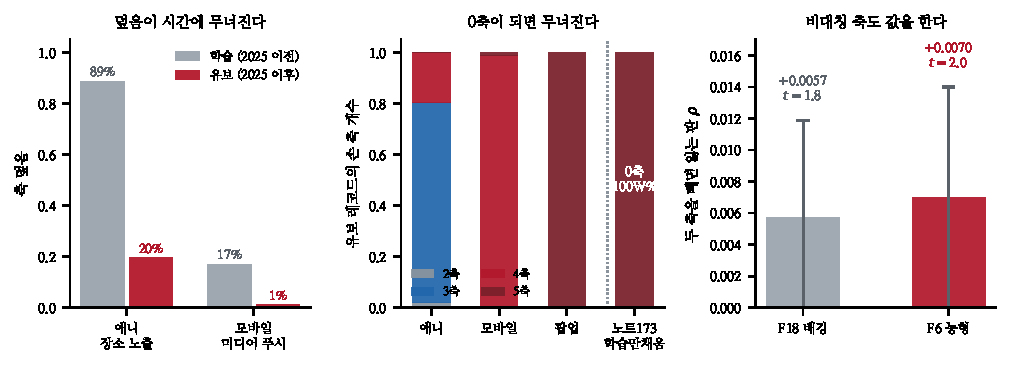
\includegraphics[width=\textwidth]{figs/bare.pdf}
\caption{왼쪽 --- 덮음이 시간에 무너진다. 가운데 --- 그래도 유보 레코드에
축이 남는다. 오른쪽 --- 비대칭 축도 값을 한다.}
\end{figure*}

\section{덮음이 시간에 무너지는 축이 둘}

\begin{table}[t]
\centering\tsize
\caption{학습 대 유보 덮음.}
\begin{tabular}{lrr}
\toprule
& 학습 & 유보 \\
\midrule
\textbf{애니 · 장소 노출} & \textbf{88.7\%} & \textbf{19.6\%} \\
모바일 · 미디어 푸시 & 17.1\% & 1.1\% \\
\bottomrule
\end{tabular}
\end{table}

모바일은 연도별로 단조다 --- 2011년 45\% · 2015년 35\% · 2020년 7\% ·
2025년 1\%. 최근 앱일수록 스크린샷 수가 안 긁힌다.

\claimx{\textbf{노트 173의 규약대로면 이 둘은 빼야 한다.} 학습에서만
쓸 수 있는 축이니 모형이 거기 기대면 예측 시점에 배신한다는 논리였다.}{애니는
판의 23\%를 차지한다 --- 규약이 옳다면 꽤 큰 손해를 보고 있는 셈이었다.}

\section{뺐더니 판이 내려간다}

\begin{table}[t]
\centering\tsize
\caption{두 축을 학습에서도 끄면.}
\begin{tabular}{lrrl}
\toprule
& 잃는 판 $\rho$ & 짝 sd & \\
\midrule
F18 배깅 & $+$.0057 & .0031 & $t{=}1.8$ \\
\textbf{F6 능형} & \textbf{$+$.0070} & .0035 & \textbf{$t{=}2.0$ 갈린다} \\
\bottomrule
\end{tabular}
\end{table}

\claimx{\textbf{규약이 틀렸다.} 훨씬 심하게 비대칭인 축을 빼면 오히려
판이 내려가고, 능형에서는 갈린다.}{하루 전에 적은 규약이다. \textbf{한
사례(팝업)에서 본 것을 규칙으로 올린 것이 성급했다.}}

\section{맨몸이 문제였다}

\begin{table}[t]
\centering\tsize
\caption{유보 레코드의 손 축 개수.}
\begin{tabular}{lrl}
\toprule
& 분포 & 0축 \\
\midrule
애니 (606) & 2축 12 · 3축 475 · 4축 119 & \textbf{없음} \\
모바일 (441) & 3축 2 · 4축 434 · 5축 5 & \textbf{없음} \\
팝업 (59) & 5축 59 & 없음 \\
\midrule
\textbf{노트 173 학습만 채움 (51)} & \textbf{0축 51} & \textbf{전부} \\
\bottomrule
\end{tabular}
\end{table}

\claimx{\textbf{문제는 비대칭이 아니라 맨몸이다.} 손 축이 하나라도 남으면
모형은 구별할 재료가 있다. 애니는 최소 2축, 모바일은 최소 3축이 남는다.
노트 173에서 무너진 51건만 0축이었다.}{그래서 애니의 장소 노출이 유보에서
80\% 빠져도 나머지 축이 그 레코드를 구별한다 --- \textbf{빠진 축이 아니라
남은 축을 봐야 했다.}}

\claimx{\textbf{규약을 좁혀 다시 적는다} --- ``유보 레코드에 손 축이 0개인
것이 있으면 안 된다.'' 가드 열둘째 \textbf{맨몸}으로 넣었고 지금 세
도메인 전부 0.0\%다.}{문턱은 10\%로 뒀다. 노트 173에서 무너진 사례가
44\%(51/116)였으니 여유가 있다 --- \textbf{그 사이 어디서 무너지는지는
안 쟀다.}}

\section{하루 만에 좁힌 것이 처음은 아니다}

\begin{table}[t]
\centering\tsize
\caption{이 흐름에서 자기 결론을 좁힌 것.}
\begin{tabular}{lll}
\toprule
세운 노트 & 좁힌 노트 & 무엇이 \\
\midrule
157 예측 & 158 & 반증 (뒤에 159가 부분 복원) \\
158 달력 $+$20\%p & 159 & $+$3\%p 로 \\
163 크기 설명 & 169 & $+$0.90이 $+$0.00 \\
165 제작사 5/5 & 166 & 복제 아티팩트 \\
\textbf{173 대칭 규약} & \textbf{174} & \textbf{맨몸 규약으로} \\
\bottomrule
\end{tabular}
\end{table}

\claimx{\textbf{규약을 세운 다음 사이클에 반례를 찾는 것이 값이 있다.}
다섯 번 중 다섯 번 다 좁혀졌고, 좁힌 뒤가 더 쓸 만하다 --- ``대칭이어야
한다''는 애니와 모바일을 잘못 버리게 했을 것이고 ``맨몸이면 안 된다''는
안 그런다.}{반대로 말하면 \textbf{한 사례에서 세운 규약은 대개 너무
넓다.} 노트 173의 팝업 하나, 노트 158의 달력 하나, 노트 163의 축 다섯 ---
전부 표본이 하나이거나 다섯이었다.}

\begin{table}[t]
\centering\tsize
\caption{남은 것.}
\begin{tabular}{ll}
\toprule
문턱 & 0축이 몇 \\%부터 무너지나 --- 안 쟀다 \\
모바일 & 스크린샷 수가 왜 최근에 안 긁히나 \\
\textbf{남은 축} & ``몇 축이 남았나''를 자질로 쓰면 \\
\bottomrule
\end{tabular}
\end{table}

마지막 줄이 곧바로 잴 수 있다. 유보 레코드마다 손 축이 몇 개 관측됐는지가
그 자체로 신호일 수 있다 --- 축이 많이 매겨진 레코드는 자료가 두꺼운
레코드이고, 자료가 두꺼운 것과 결과가 큰 것이 붙어 있을 수 있다.
\textbf{그러면 그것은 자질이 아니라 누수다.}

\end{document}
